In this section, we compare STRUCT to a state-of-the-art NLG system,
CRISP~\footnote{We considered using the PCRISP system as a
  baseline~\cite{bauer_sentence_2010}. However, we could not get it to
  work, and we did not receive a response to our queries, so we were
  unable to use it.} 
and evaluate three hypotheses: (i) STRUCT will be
comparable in speed and generation quality to CRISP as it generates
increasingly large referring expressions, (ii) STRUCT will be
comparable in speed and generation quality to CRISP as the size of the
grammar which they use increases, and (iii) STRUCT is capable of
communicating complex propositions, including multiple concurrent
goals, negated goals, and nested subclauses.
Finally, we evaluate the effect on STRUCT's performance 
of varying key parameters, including grammar size.

\section{Comparison to CRISP}
% Input to STRUCT comes in two parts: a
% grammar file and a world file. The grammar file contains a list of
% elementary trees and a lexicon.  The elementary trees may be either
% initial or adjoining trees, and have semantic roles of arguments
% clearly marked, while the lexicon entries reference these elementary
% trees and lexicalize them.  These lexicon entries also refer to the
% semantic meanings and semantic requirements of the trees which they
% represent.  All this information is encoded in our grammar (for these
% experiments, we use a deterministic grammar, as CRISP does). World
% files also contain a list of communicative goals, which are
% automatically encoded into a reward function by STRUCT.  Our reward
% function gives 50 points for using the correct communicative goal, and
% an additional $10 + \frac{20}{n}$ points for a correct reference to an
% argument, where $n$ is the number of other entities that are possible
% referents for the argument.

We first describe experiments comparing STRUCT to CRISP. We used a
2010 version of CRISP  which uses a Java-based GraphPlan
implementation. In these
experiments, we use a deterministic grammar.  Our reward function
gives 50 points for using the correct communicative goal, and an
additional $10 + \frac{20}{R}$ points for a correct reference to an
argument, where $R$ is the number of other entities that are possible
referents for the argument. Because the reward signal is fine-grained,
 a myopic action selection strategy is
sufficient for these experiments, and 
the $d$ parameter is set to zero. The
number of simulations for STRUCT varies between 20 to 150.
In most cases, a small $n$, under 100, is sufficient
to guarantee generation success.  The exploration constant $c$ in
Equation~\ref{eqn:uct} is irrelevant when $n \leq |\bf{A}|$, since it
applies only to actions selected after all open actions have already
been tried once.

\begin{figure}
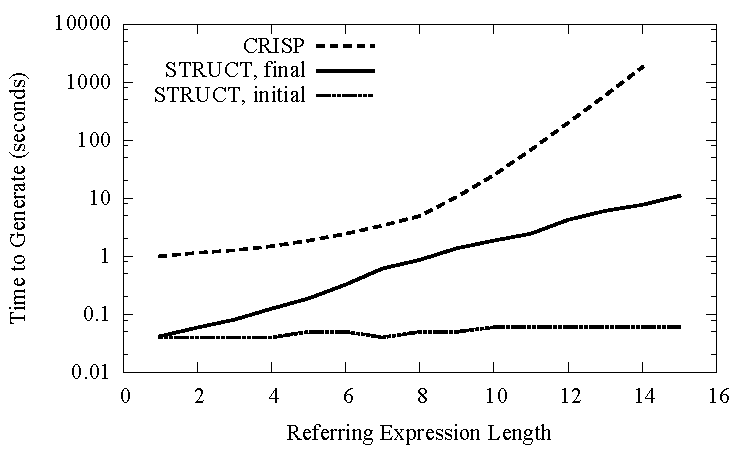
\includegraphics[width=0.7 \linewidth ]{../analysis/plots/complex-goal/complex-goal.pdf}
\caption{Experimental comparison between STRUCT and  CRISP: 
Generation time vs. length of referring expression }
\label{crisp-comparison-gentime}
\end{figure}

\begin{figure}
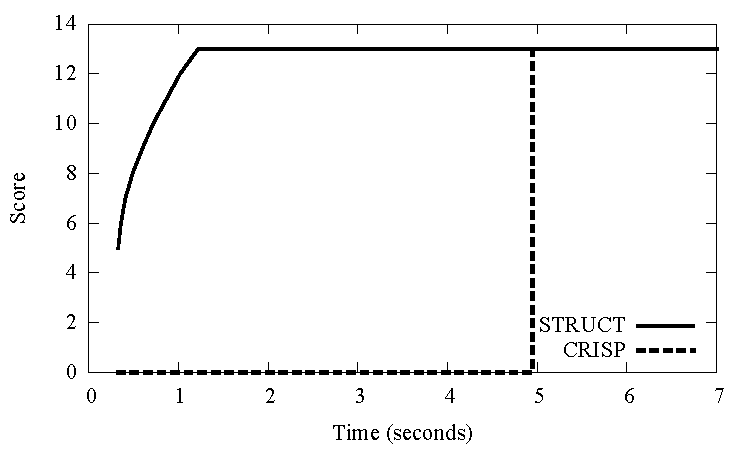
\includegraphics[width=0.7 \linewidth ]{../analysis/plots/complex-goal/complex-goal-anytime.pdf}
\caption{Experimental comparison between STRUCT and  CRISP:
Score of best solution vs time.}
\label{crisp-comparison-score}
\end{figure}

\subsection{Comparison to CRISP: Referring Expressions}
We first evaluate CRISP and STRUCT on their ability to generate
referring expressions. We follow prior work (\cite{koller_experiences_2011})
in our initial experiment design.  We consider a series of sentence
generation problems which require the planner to generate a sentence
equivalent to ``The Adj$_1$ Adj$_2$ ... Adj$_k$ dog chased the cat.",
where the string of adjectives is a string that distinguishes one
dog (whose identity is specified in the problem description) from
all other entities in the world.
The experiment has two parameters: $j$, the number of adjectives in
the grammar, and $k$, the number of adjectives necessary to
distinguish the entity in question from all other entities. We set $j
= k$ and show the results in Figure~\ref{crisp-comparison} (a).
We observe that CRISP was able to achieve
sub-second or similar times for all expressions of less than length 5, but its
generation times increase exponentially past that point, exceeding 100
seconds for some plans at length 10. At length 15, CRISP failed to
generate a referring expression; after 90 minutes the Java garbage
collector terminated the process. STRUCT, performs much better and
is able to generate much longer referring expressions without failing.
Later experiments had successful referring expression generation of lengths
as high as 25.

We can also observe the anytime nature of STRUCT from this experiment,
shown in Figure~\ref{crisp-comparison} (b).  Here we look at the
length of the solution sentence generated as a function of time, for
$k=8$, a mid-range scenario which both generators are able to solve
relatively quickly ($< 5s$).  As expected, CRISP produces nothing until
the end of its run, at which point it returns the solution. STRUCT,
however, quickly produces a reasonable solution, ``The dog chased the
cat.''  This is then improved upon by adjoining until the referring
expression is unambiguous. If at any point the generation process was
interrupted, STRUCT would be able to return a solution that at least
partially solves the communicative goal.

\begin{figure}
\centering
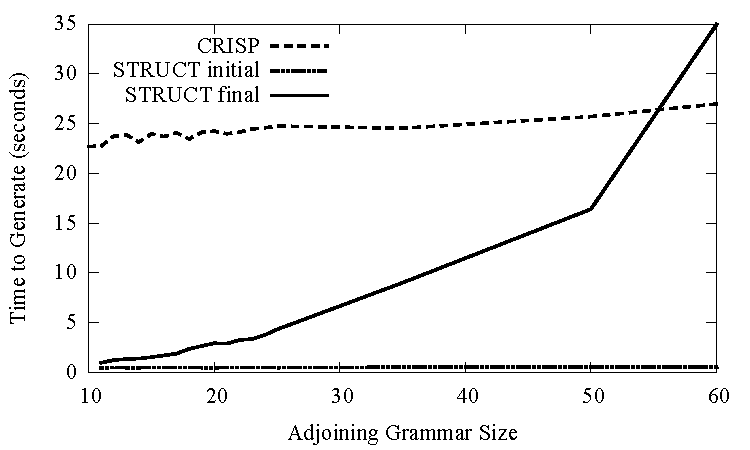
\includegraphics[width=0.7 \linewidth]{../analysis/plots/large-grammar/large-grammar.pdf}
\label{graph-large-grammars}
\caption{Effect of grammar size}
\end{figure}

\begin{figure}
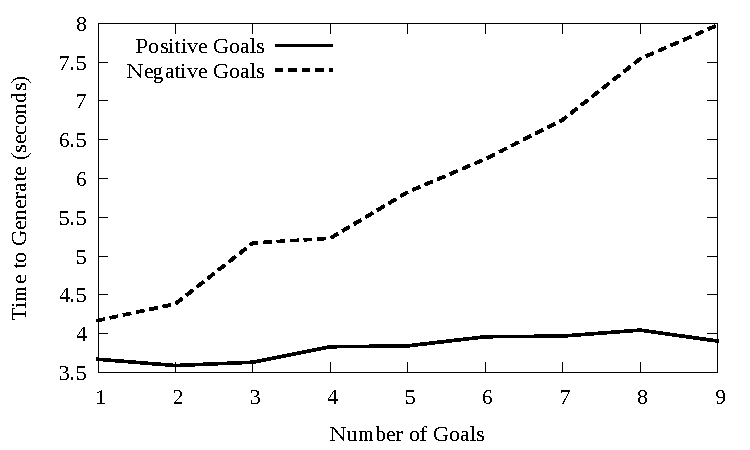
\includegraphics[width=0.7 \linewidth]{../analysis/plots/goals/differentgoals.pdf}
\label{chart-different-goals}
\caption{Effect of multiple and negated goals}
\end{figure}

\begin{figure}
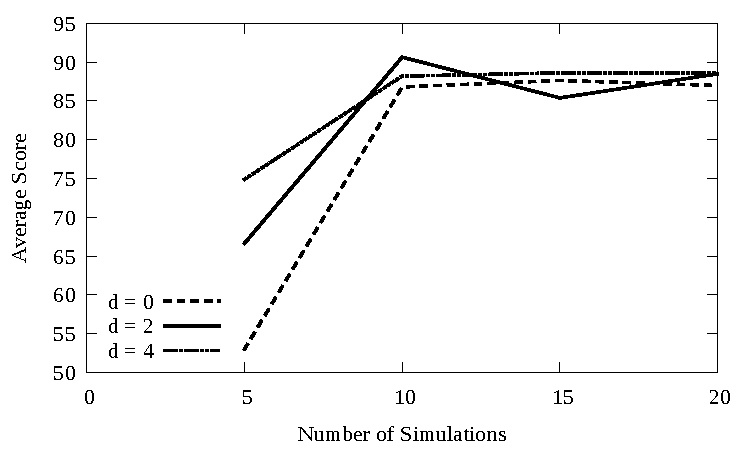
\includegraphics[width=0.7 \linewidth]{../analysis/plots/params/pltag-n-v-score.pdf}
\label{chart-n-v-score}
\caption{Effect of parameter variations on the STRUCT solution.}
\end{figure}


\subsection{Comparison to CRISP:  Grammar Size}
We next evaluate STRUCT and CRISP's ability to
handle larger grammars. This experiment is set up in the same way as
the one above, with the exception of $l$ ``distracting'' words, words
which are not useful in the sentence to be generated.  $l$ is defined
as $j - k$.  In these experiments, we vary $l$ between 0 and 50.
Figure~\ref{graph-large-grammars} shows the results of these
experiments.  We observe that CRISP using GraphPlan, as previously
reported in \cite{koller_experiences_2011}, handles an increase in
number of unused actions very well.  Prior work reported a difference
on the order of single milliseconds moving from $j = 1$ to $j = 10$.
We report similar variations in CRISP runtime as $j$ increases from 10
to 60: runtime increases by approximately 10\% over that range.

STRUCT's performance with large grammars is similar to CRISP using the
FF planner \cite{hoffmann_ff_2001}, also profiled in
\cite{koller_experiences_2011}, which increased from 27 ms to 4.4
seconds over the interval from $j = 1$ to $j = 10$.  STRUCT's
performance is less sensitive to larger grammars than this, but over
the same interval where CRISP increases from 22 seconds of runtime to
27 seconds of runtime, STRUCT increases from 4 seconds to 32 seconds.
This is due almost entirely to the required increase in the value of
$n$ (number of samples) as the grammar size increases.  At the low
end, we can use $n=20$, but at $l = 50$, we must use $n = 160$ in
order to ensure perfect generation as soon as possible.  Fortunately,
as STRUCT is an anytime algorithm, valid sentences are available very
early in the generation process, despite the size of the set of
adjoining trees (the ``STRUCT Initial'' curve in
Figure~\ref{graph-large-grammars}).  This value does not change
substantially with increases in grammar size.  However, the time to
improve this solution does. An interesting question for future work is
how to limit this increase in time complexity in STRUCT. 

\section{Evaluation of Complex Communicative Goals}
In the next set of experiments, we illustrate that STRUCT can solve
conjunctions of communicative goals as well as negated communicative goals.

\subsection{Multiple Goals}
We next evaluate STRUCT's ability to accomplish
multiple communicative goals when generating a single sentence.  In this
experiment, we modify the problem from the 
previous section.  In that section, the referred-to dog was unique,
and it was therefore possible to produce a referring expression which
identified it unambiguously.  In this experiment, we remove this
condition by creating a situation in which the generator will be
forced to ambiguously refer to several dogs.  We then add to the
world a number of adjectives which are common to each of these
possible referents.  Since these adjectives do not further
disambiguate their subject, our generator should not use
them in its output.  We then encode these adjectives into
communicative goals, so that they will be included in the output of
the generator despite not assisting in the accomplishment of
disambiguation.  We find that, universally, these otherwise useless
adjectives are included in the output of our generator, demonstrating
that STRUCT is successfully balancing multiple communicative goals.
As we show in figure \ref{chart-different-goals} (the ``Positive
Goals'' curve) , the presence of additional satisfiable semantic goals does
not substantially affect the time required for generation.  We are able to
accomplish this task with the same very high frequency as the CRISP
comparisons, as we use the same parameters.

\subsection{Negated Goals}
We now evaluate STRUCT's ability to generate
sentences given negated communicative goals.  We again modify
the problem used earlier by 
adding to our lexicon several new adjectives, each applicable only to
the target of our referring expression.  Since this entity can now be
referred to unambiguously using only one adjective, our generator
should just select one of these new adjectives.  We then encode these
adjectives into negated communicative goals, so that they will not be
included in the output of the generator, despite allowing a much
shorter referring expression.  We find that these adjectives which
should have been selected immediately are omitted from the output, and
that the sentence generated is the best possible under the
constraints.  This demonstrates that STRUCT is balancing these negated
communicative goals with its positive goals.  Figure
\ref{chart-different-goals} (the ``Negative Goals'' curve) shows the
impact of negated goals on the time to generation.  Since this
experiment alters the grammar size, we see the time to final
generation growing linearly with grammar size.  The increased time to
generate can be traced directly to this increase in grammar size.

\subsection{Effect of Parameters}
Finally, we study the effect of the number of simulations and
lookahead depth on the performance of STRUCT. We design this
experiment to require lookahead by using  a sparse
reward function that penalizes a final sentence based on the number of
adjectives it has. We also use a probabilistic LTAG that has multiple
actions all relevant to reaching the goal, but that add differing
numbers of adjectives to the sentence. We then run STRUCT on this
problem with differing parameter values and report the score of the
best solution found, as measured by our reward function
(Figure~\ref{chart-n-v-score}). 

From the figure, it is clear that as the number of simulations
increase, the quality of the solution improves for all values of $d$.
This is likely because increasing simulations means a better estimate
of the utility of each action. Further, in this particular case,
increasing the depth of lookahead also yields a benefit, because of
the structure of our problem. This is especially true if the branching
factor of the search space is large, which is common in NLG
applications.  Similarly, the deeper we allow the tree search to continue, the
better the estimation of the future value of each action,
especially since actions have far-reaching consequences for the
meaning of the sentence at its conclusion. 
It is interesting that even for low numbers of
simulations $d=4$ is able able to find a reasonably good
solution. These behaviors are expected and verify 
that STRUCT does not display any pathologies with respect to its parameters.